\chapter{La conformité dans le secteur bancaire}
\section*{Introduction}
Dans ce chapitre, nous élaborerons d’abord une étude de l'existant. Pour celà, 
nous présenterons quelques plateformes permettant d'analyser 
des opérations de transferts de fonds. Après cela, Nous étudierons la fonction conformité ou 
compliance en anglais dans le secteur bancaire. 


\section{Etude de l'existant}
\subsection{Analyse des dossiers de transfert à la SGBF}

Le problème posé au niveau du service OPI, c'est l'analyse en temps réel des
dossiers de transferts reçus au niveau du guichet. Cette analyse suit un
processus.
La première phase de ce processus est la réception du dossier.
A la réception du dossier, le collaborateur analyse la cohérence du dossier.
Cette analyse consiste en la vérification de la cohérence et l'exactitude des
informations contenues sur les éléments constitutifs du dossier.

Après cette phase, le collaborateur analyse la complétude du dossier. Une fiche,
disponible au niveau du guichet permet aux collaborateurs de OPI de savoir à vue
d'oeil quels justificatifs devraient être présent dans le dossier en fonction du
motif de l'opération.

L'étape suivante est la vérification de la fiabilité des différents acteurs de l'opération
à travers des outils comme Force-online.

La dernière étape concerne la vérification du circuit de transfert. Il s'agit à cette étape
de s'assurer que la règlementtion autorise l'opération qui est entrain d'être menée entre les diffrents acteurs.

\subsection{Plateformes existantes dans le milieu bancaire}

De nombreuse plateformes permettent de juger le risque de non-conformité d'un acteur d'une
opération de transfert. Ces plateformes sont toutes propriétaire.

\subsubsection{ComplianceBond}

\textbf{ComplianeBond} est un des produits de la plateforme HighBond. HighBond
est une plateforme logicielle de gouvernance d'entreprise qui renforce la 
sécurité, la gestion des risques, la conformité et l'assurance. ComplianceBond
est une solution de gestion de la conformité qui permet aux organisations de
mettre en oeuvre, d'automatiser et de démontrer une assurance par rapport à un
programme de conformité.

Les fonctionnalités principales de ComplianceBond sont les suivantes:
\begin{itemize}
  \item Centraliser la documentation des besoins et des contrôles mappés. Cela
    permet de réduire le temps passé à documenter et à tester la conformité.
  \item Evaluer et surveiller la conformité en automatisant les tests de
    surveillance de conformité en temps réel.
  \item Rapport sur le statut de conformité
\end{itemize}
Il s'agit d'une plateforme propriétaire.

\subsubsection{TraProtect} 

TraProtect de TraInvestment est une plate-forme multicanal, multi-activité et
multi-niveau de prévention temps réel et détection de la fraude des 
transactions spécialement conçue pour le monitoring des transactions de 
paiement électronique. Elle est destinée à toute institution traitant les 
transactions de paiement électronique.

\subsubsection{ kdprevent}

La plateforme kdprevent permet de lutter contre le blanchiment d'argent et le 
financement du terrorisme. Elle a été mise en œuvre dans plusieurs pays du 
monde, dans plus de 50 institutions. Elle  est conçue pour détecter les 
activités inhabituelles, inattendues et suspectes. Une fois détectée, elle 
envoie automatiquement des avertissements aux responsables, généralement les 
responsables conformité.
Ses principales fonctionalités sont:
\begin{itemize}
  \item Analyse d'une transaction unique et d'un ensemble de transactions 
    liées qui ont eu lieu dans une période de temps donnée.
  \item Détection automatique et interruption des transactions suspectes
    (i.e SWIFT, SEPA, SIC, etc.) et notification en temps réel.
  \item Génération d'alertes pour les situations suspectes détectées
  \item Un analyseur de relations qui vous permet d'explorer les relations 
    potentiellement suspectes ou inconnues qui existent entre les clients,
    les emprunteurs ou les comptes.
\end{itemize}


\section{La conformité ou compliance}

Le cadre règlementaire autour des activités financières a été fortement
renforcé, faisant de la conformité (ou Compliance) un pilier indispensable
de la protection des institutions financières en particulier les banques 
et de leurs clients. \cite{arnaud2015}

  \begin{figure}[h!]
    \begin{center}
      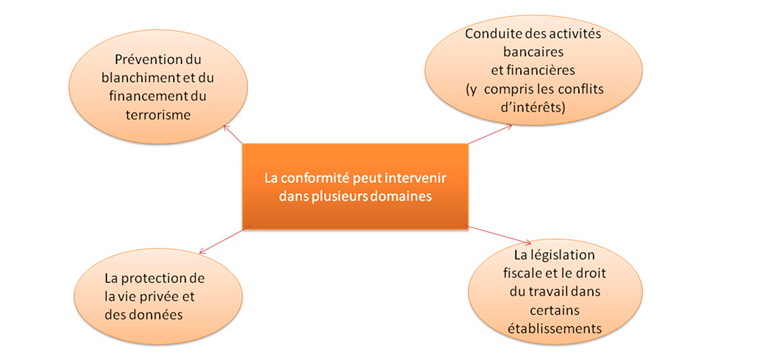
\includegraphics[width=14cm]{images/domaineconformite.png}
        \caption{Domaine d'intervention de la conformité
        .\label{fig:domaineconformite}}
    \end{center}
  \end{figure}

\subsection{Définition}
La conformité en anglais compliance est un concept qui a fait naître de 
nouvelles obligations pour le banquier. En effet, face à la complexité des
environnements et à \og l'inflation règlementaire\fg,  la fonction 
conformité a pour but de prévenir tout risque de non-conformité des opérations
bancaires et financières. La conformité se définit donc comme l’obligation 
de veiller à ce que les collaborateurs des différentes banques s’assurent en
permanence que soient respectées:
\begin{itemize}
  \item Les dispositions législatives et règlementaires propres aux activités
    bancaires;
  \item Les normes et usages professionnels et déontologiques ;
   \item Les codes de conduites notamment le code éthique et les procédures internes
\end{itemize}

Dans ses grandes lignes, la conformité consiste à:
\begin{itemize}
  \item Identifier et à jauger le degré de non-conformité d’une entité 
    économique par rapport à l’ensemble des règles de conduite qui lui sont
    applicables
  \item Mesurer son taux d’exposition aux risques de sanction judiciaire et
    administrative
  \item Evaluer les pertes financières qu’elle pourrait subir
  \item Conseiller une entité économique pour qu’elle se mette en 
    conformité avec les normes législatives et règlementaires.
\end{itemize}

En somme, la conformité est l’ensemble des actions visant
à l’intégration, dans la structure bancaire des exigences issues des 
règlementations financières.  La fonction conformité dans une banque
recouvre quatre grandes activités :

\subsubsection{Sécurité financière}
Elle est attentive à la sécurité financière de la banque et lutte en ce sens 
contre la fraude, le blanchiment de capitaux et financement du terrorisme, 
les abus de marché et les embargos.

\subsubsection{La protection Clientèle}
Elle assure en parallèle, une protection continue de la clientèle en
préservant aussi bien leurs intérêts propres, que ceux des marchés ou de la 
banque elle-même.

\subsubsection{Le contrôle permanent}

Elle appartient au dispositif global de contrôle permanent et assure la
gestion des risques de non-conformité.

\subsubsection{La déontologie}

La déontologie est également une partie intégrante de la conformité. Elle
permet de s’assurer du respect du recueil des règles de déontologie de 
l’établissement bancaire ainsi que de traiter les signalements pouvant 
provenir de tous les collaborateurs de la banque.

\subsection{Rôle de la conformité dans le domaine bancaire}

Le rôle de la conformité est d’abord de donner aux dirigeants de la Banque 
ainsi qu’au Conseil d'administration l'assurance raisonnable que les risques 
de non-conformité réglementaires et de réputation sont dûment surveillés, 
contrôlés et atténués au niveau du Groupe. C’est également s'assurer en 
permanence que les lois et réglementations ainsi que les règles et normes 
internes définies par les pays sont respectées. In fine, il s’agit d’offrir 
aux clients l’assurance d’un environnement sécurisé pour réaliser leurs 
opérations financières, en vérifiant que celles-ci sont conformes aux règles 
déontologiques et aux législations.

\section{Présentation du cadre règlementaire}

La SGBF est membre d'un groupe international français. Elle est donc soumise
aussi bien aux règlements de la zone UEMOA qu'à celles européennes et 
internationales.

Au niveau international, l'organisme de référence de contrôle est le GAFI.
Le GAFI (Groupement d'Action FInancière) est un organisme international, sous
l'égide des nations unies, créé à Paris en  1989. Il a pour rôle d'émettre des
recommandations dans le domaine de la lutte contre le blanchiment des capitaux
et dans la lutte contre le financement du terrorisme. Les pays membres du GAFI
acceptent de fait les recommandations et s'engagent à mettre en oeuvre les lois
permettant l'application de ces recommandations. Les pays membres du GAFI
s'engagent également à s'auto-évaluer à intervalles de temps réguliers dans le
but d'améliorer leurs dispositifs respectifs.
Il s'agit aujourd'hui la référence principale dans le domaine de l'AML (Anti
Money Laundering).

Les contrôles de la fonction conformité regroupent aussi bien ceux sur la
règlementation de change que ceux sur les composantes d'un programme AML
\nomenclature{AML}{Anti Money Laundering}.

\subsection{ La règlementation de change} 

La règlementation de change est un outil juridique important non seulement
dans le monde des affaires, mais aussi dans la vie d’un pays compte tenu de
la diversité des phénomènes économiques et de la criminalité qui pourrait
se développer dans ce domaine. Elle relève de la tutelle du Ministre chargé
des Finances. Elle prescrit que les règlements financiers et mouvements de 
capitaux entre l'UEMOA et l'Etranger, ainsi que les opérations de change manuel
dans l'UEMOA, ne peuvent s'effectuer que par l'entremise de la BCEAO ou d'une 
banque intermédiaire agréé\cite{reglementfin}.

Le Change se définit comme l’échange d’une monnaie contre une autre, C’est le 
bénéfice réalisé sur la différence des cours entre deux monnaies. C’est aussi 
le taux de conversion entre deux monnaies.

Au Burkina Faso et dans les pays membres de l’UEMOA, les transferts à 
l’étranger sont régis par un ensemble de texte. Ces textes fixent les 
procédures à suivre par les intermédiaires agréés en matière d’exécution des
opérations avec l’étranger et déterminent la procédure de domiciliation et de 
règlement des importations par la banque.

\subsubsection{La règlementation de change sur les opérations d'exportation}

Les opérations d'exportations d'un montant supérieur à 500000 sont soumises à
domiciliation auprès d'une banque. Pour chaque opération 
d'exportation, les résidents sont tenus d'encaisser les recettes en devises 
et de les céder à la banque domiciliataire dans un délai d'un mois à compter
de la date d'exigibilité du paiement.
 
\subsubsection{La règlementations de change sur les opérations d'importation}

Les opérations d'importation de marchandises étrangères, c'est-à-dire originaires
d'un pays extérieur à la zone franc, doivent être domiciliées auprès d'une banque
intermédiaire agréé, lorsque leur valeur dépasse un certain seuil variable selon 
les pays.\cite{reglementfin}
Pour une opération d'importation, le dossier complet de domiciliation doit contenir
une copie de la facture établi par le fournisseur, une attestation d'importation,
et un formulaire d'autorisation de change.
 
\subsubsection{La règlementation de change sur les opérations d'investissement et
d'emprunt}
La règlementation de change exige que pour tout investissement, prêt, ou
opération en capital par un résident, une autorisation préalable du ministère
chargé des finances est obligatoire.
 
\subsection{Les composantes d'un programme AML}

Les programmes AML permettent de garantir la sécurité financière d'un
établissement financier. Ce sont:
 \begin{enumerate}
   \item Lutte contre le blanchiment des capitaux
     (AML/LAB)\nomenclature{LAB}{Lutte Anti Blanchiment}
   \item Lutte contre le financement du terrorisme
     (CFT)\nomenclature{CFT}{Contre le Financement du Terrorisme}
   \item Respect des embargos commerciaux et financiers
   \item Surveillance des opérations de marché
 \end{enumerate}
 
 \subsubsection{La lutte contre le blanchiment de capitaux} 

\textbf{Le blanchiment de capitaux} consiste à dissimuler la provenance d'argent acquis
de manière illégale, appelé communément \og{}argent sale\fg{}, en lui donnant
l'apparence de fonds d'origine licite(\og{}argent propre\fg{}) pour le
réinvestir dans des activités légales.
Le Blanchiment permet notamment aux criminels de masquer une augmentation
trop ostensible de leur richesse afin d'éviter d'attirer l'attention des autorités.
On distingue trois phase dans le processus global de blanchiment:
\begin{description}
  \item[\textbf{La phase de placement}] qui consiste à injecter dans le système financier
    les sommes d'argent issues des crimes et des délits; 
  \item[\textbf{La phase d'empilement}] qui consiste à brouiller les pistes. Le but est 
    d'effectuer un ensemble de transactions qui ont pour objectif d'empêcher 
    toute traçabilité des mouvements de fonds pour remonter à l'opération 
    d'origine.
  \item[\textbf{La phase d'intégration}] qui consiste à réinvestir les fonds
    dans des placements honorables: biens immobiliers, titres, participations
    financires dans les entreprises.
\end{description}

Lutter contre le blanchiment de capitaux reviendrait donc à mettre 
en place des mesures d vigilance au niveau des acteurs sociaux et économiques
pour que les étapes à franchir pour blanchir les capitaux soient difficiles
voire impossible. \cite{reglementaml}

\subsubsection{La lutte contre le financement du terrorisme}

\textbf{Le financement du terrorisme} consiste à fournir ou réunir des fonds,
des biens ou des services susceptibles d'être utilisés dans le but de facilité
ou de perpétrer des actes de terrorisme.
Ces opérations à finalité criminelle impliquent parfois des fonds d'origine
parfaitement légale.
Alors que le blanchiment des capitaux est une opération financière qui vise 
à cacher l'origine des fonds, le  financement du terrorisme, au contraire,
utilise des techniques pour tenter de cacher la destination des fonds.

La lutte contre le financement du terrorisme s'effectue par identification et
contrôle du donneur d'ordre, du destinataire effectif de la transaction, et 
ceci par filtrage par rapport à des listes de sanctions officielles.

\subsubsection{Le respect des embargos commerciaux et financiers}

La communauté internationale, au travers de l'Organisation des Nations Unies 
(ONU), s'est dotée d'un arsenal juridique pour permettre le contrôle des flux
monétaires. Parmi certaines mesures figure l'embargo commercial. \textbf{Un embargo} 
(généralement partiel), vise à restreindre les relations des pays membres
avec le pays concerné et à encadrer strictement ce qu'il est permis de faire
ou non en matière de commerce et d'échange. Les embargos se traduisent 
généralement par des mesures d'interdiction de certains types d'opérations, 
comme par exemple l'interdiction de commercer sur du matériel d'origine 
nucléaire ou militaire, ou encore l'interdiction d'exporter les ressources 
pétrolières d'un pays sous embargo.

\subsubsection{La surveillance des opérations de marché}

Il s'agit d'une obligation qui vise à s'assurer que la banque ou l'établissement
financier n'utilise pas son accès privilégié aux marchés financier pour en tirer
profit au détriment de ses clients. La surveillance des marchés regroupe les
fonctions suivantes:
\begin{description}
  \item[Les délits d'initiés:]
    Pratique consistant à profiter indument d'une information privilégiée avant
    que celle-ci ne soit rendue publique. Une information privilégiée est une 
    information précise sur un émetteur qui, si elle était rendu publique, 
    serait susceptible d'influencer le cours de certains instruments 
    financiers.
  \item[Les manipulation de marché: ]
    Cette problématique vise à s'assurer que la banque ou l'établissement 
    financier n'utilise pas son poids financier et son effet de levier sur 
    certains titres pour faire évoluer le marché dans un sens qui lui est 
    favorable. 
  \item[La résolution des conflits d'intérêts: ]
    Cette dernière problématique vise à identifier les éventuels conflits 
    résultant de la multiplicité des activités bancaires au sein d'un grand
    groupe financier.
\end{description}

\section{Machine Learning et mise en oeuvre d'un programme de conformité}

Après avoir présenté les composantes d'un programme AML, nous allons analyser
les moyens à mettre en oeuvre au sein des établissements de crédit pour 
appliquer de manière opérationnelle les recommandations du GAFI
\nomenclature{GAFI}{Groupe d'Action FInancière} et surtout 
comment ces moyens pourraient être automatisés grâce au ML.
 
\subsection{Le Machine Learning pour la simplification des procédures KYC}
 
KYC \nomenclature{KYC}{Know Your Customer} est l'acronyme de Know Your Customer. Il désigne le processus permettant 
de vérifier l'identité des intervenants à une opération bancaire afin de 
s'assurer de la conformité des clients face aux législations anti-corruption,
de leur probité et de leur intégrité.

Initialement mise en oeuvre par une intervention humaine, les tâches 
répétitives des procédures KYC pourraient être automatisées grâce au 
Machine learning. Les principales étapes de la procédure KYC qui peuvent être
automaisées par des modèles d'apprentissage automatiques sont:
  
  \subsubsection{L'identification et le contrôle des informations 
    d'identification des clients}
    Il s'agit au cours de cette étape de demander et d'enregistrer les
    informations personnels du clients et de contrôler son identité par rapport
    à une pièce d'identité officielle. A ce niveau, les informations
    personnelles nom, prénoms, date de naissance, situation maritale,
    adresse\ldots dites \og bio data \fg sont demandées.

    Le contrôle des informations d'adresse nécessitera la fourniture par le 
    client d'une pièce probante (facture d'eau, de téléphonie fixe, etc.).
    La banque pourra également adresser un courrier de bienvenue ou de 
    remerciement pour la fidélité au client  et vérifier que le courrier ne
    revient pas.

  \subsubsection{Le contrôle des clients par rapport aux listes de sanctions}
    Lors de toute opération, la banque contrôle la présence éventuelle d'un
     des intervenants de l'opération sur une ou plusieurs listes de 
    sanction, selon la réglementation en vigueur dans le pays. Ces listes sont
    établies par les autorités officielles(nationales ou supranationales comme
    L'ONU, L'Union Européenne). Elles regroupent des individus ou de groupes qui
    compte tenu de leur activités ont été frappé de mesure d'embargo nominative.

  \subsubsection{Qualification du risque de blanchiment}
    Il s'agit là de vérifier si le client n'existe pas sur des listes qui ne 
    sont pas d'ordre public. Ces listes peuvent être celles des PEP
    \nomenclature{PEP}{Personnes Exposées Politiquement} ou une liste d'indésirables car en opposition 
    avec la déontologie et les valeurs du groupe financier.

  \subsubsection{Consignation des pièces d'identification des clients}
    Après la phase d'identification du client et de son contrôle, 
    l'établissement financier doit enregistrer les preuves d'identification du
    client et les archiver.

    
\subsection{Le Machine Learning, un outil essentiel à la détection des 
 transactions suspectes}
 
 La lutte contre le blanchiment d'argent et le financement du terrorisme est
 principalement basée sur l'élaboration, par des algorithmes, de scénarios
 d'anticipation dits « déterministes ». Les algorithmes utilisés analysent
 en temps réel les transactions et sont capables, en quelques instants, de
 décéler une transaction suspecte. Ces scénarios se basent sur des règles
 arrêtées, constantes et ne sont que très peu modifiés une fois mis en 
 place. La procédure est basé sur des mots clés et il est difficile de calibrer
 ces logiciels à un niveau permettant une protection optimale face aux 
 transactions frauduleuses sans générer pour autant un nombre élevé de fausses
 alertes qui de ce fait viendrait perturber les activités de conformité.

 Pour résoudre ces problémes particulièrement chronophages et coûteux pour les
 banques, des applications basées sur le Machine Learning pourraient apprendre
 à identifier les transactions frauduleuses en établissant des procédés 
 standardisés et automatisés. Cela permettra de réduire la charge de travail des
 équipes, tout en affinant la précision de l'analyse. Il s'agirait là pour les
 banques de réduire leurs coùts et leur sanctions, tout en assignant un travail
 à plus forte valeur ajoutée aux équipes chargées de la conformité.


\section*{Conclusion}
Le blanchiment d'argent, la lutte contre le terrorisme sont des fléaux dangereux
et il est du devoir des banques de lutter efficacement contre ces pratiques. Aux
collaborateurs de la SGBF, il est demandé de:
\begin{itemize}
  \item Appliquer impérativement la règlementation française(exigence du groupe)
  \item se conformer à la règlementation du Burkina Faso applicable à leur
    égard. Si Celle-ci est plus restrictive, elle s'applique en priorité tout en
    restant conforme avec les autres exigences du groupe.
  \item Appliquer la règlementation américaine pour toute
    transaction vers les Etats-Unis ou impliquant le dollar Américain.
\end{itemize}

Ce chapitre nous a permis de présenter la conformité dans le domaine bancaire,
et les facilités qu'apporterait l'apprentissage automatique dans sa mise en 
oeuvre dans un établissement financier. La suite sera
consacrée à l'implémentation et à la présentation des résultats.

